\newpage

\section{Κεφάλαιο 6: Serverless Υπολογισμοί και λογική αυτοματοποίησης}

Όχι κάθε λειτουργία του συστήματος χρειάζεται μόνιμα ενεργό υπολογιστικό πόρο. Το παρόν κεφάλαιο παρουσιάζει την υλοποίηση μιας \textit{serverless} συνάρτησης, που ενεργοποιείται αποκλειστικά όταν συμβαίνει ένα συγκεκριμένο γεγονός, και αποδεσμεύει πλήρως τους πόρους της όταν δεν χρησιμοποιείται --- καθώς και ένα πραγματικό πρόβλημα που προέκυψε κατά την υλοποίηση, η διάγνωση και επίλυση του οποίου αποδεικνύει στην πράξη τις ιδιαιτερότητες του \textit{event-driven} προγραμματιστικού μοντέλου.
Σκοπός: Event-driven λειτουργίες για οικονομία πόρων.


\subsection{Εγκατάσταση \textit{serverless} πλατφόρμας: \textit{Knative}}

Για την υλοποίηση \textit{serverless} υπολογισμού επιλέχθηκε το \textit{Knative Serving}, αντί εναλλακτικών όπως το \textit{OpenWhisk} ή υπηρεσίες \textit{managed} \textit{serverless} δημόσιου \textit{cloud} (π.χ. \textit{AWS Lambda}). Η επιλογή αυτή έγινε επειδή το \textit{Knative} λειτουργεί \textbf{εντός} του υπάρχοντος \textit{Kubernetes cluster} (\textit{MicroK8s}), χωρίς να απαιτεί ξεχωριστή υποδομή ή εξάρτηση από συγκεκριμένο πάροχο \textit{cloud}, διατηρώντας έτσι τη συνολική αρχιτεκτονική συνεπή με τις υπόλοιπες υπηρεσίες του συστήματος, οι οποίες ήδη λειτουργούν ως πόροι \textit{Kubernetes}. Το \textit{OpenWhisk} θα απαιτούσε ξεχωριστό \textit{cluster} ή \textit{namespace} αφιερωμένο στη διαχείρισή του, ενώ το \textit{AWS Lambda} θα εισήγαγε εξάρτηση από συγκεκριμένο πάροχο (\textit{vendor lock-in}) και πρόσθετη πολυπλοκότητα δικτύωσης για την επικοινωνία με το \textit{MinIO}, το οποίο παραμένει αυτο-φιλοξενούμενο εντός του \textit{cluster}.

Η ενεργοποίηση του \textit{Knative} πραγματοποιήθηκε ως πρόσθετο (\textit{addon}) του \textit{MicroK8s}, αυτοματοποιημένη μέσω αφιερωμένου \textit{role} του \textit{Ansible}:

\begin{lstlisting}[language=yaml, caption={Ansible tasks για την ενεργοποίηση των MicroK8s addons}]
- name: Enable MicroK8s community addons repository
  command: microk8s enable community

- name: Enable MicroK8s Knative addon
  command: microk8s enable knative
\end{lstlisting}


\subsection{Σχεδιασμός \textit{triggering} μηχανισμού}

Η ενεργοποίηση της \textit{serverless} συνάρτησης βασίζεται στον μηχανισμό ειδοποίησης γεγονότων (\textit{event notification}) του \textit{MinIO}: κάθε φορά που αποθηκεύεται νέο αντικείμενο σε συγκεκριμένο \textit{bucket}, το \textit{MinIO} αποστέλλει αυτόματα \textit{webhook} ειδοποίηση προς προκαθορισμένο \textit{endpoint} --- στην προκειμένη περίπτωση, προς τη διεύθυνση της συνάρτησης \textit{Knative}:

\begin{lstlisting}[language=yaml, caption={Εγγραφή event notification στον MinIO client}]
mc event add myminio/knative-demo \
  arn:minio:sqs::thumbnailfunction:webhook \
  --event put
\end{lstlisting}

Το \textit{Knative Serving} αναλαμβάνει τη διαχείριση του κύκλου ζωής της συνάρτησης: όταν δεν υπάρχει εισερχόμενη κίνηση για ορισμένο διάστημα, το \textit{Knative} μειώνει τον αριθμό των αντιτύπων (\textit{replicas}) στο μηδέν (\textit{scale-to-zero}), αποδεσμεύοντας πλήρως τους υπολογιστικούς πόρους. Με την άφιξη νέου γεγονότος, δημιουργείται αυτόματα νέο αντίτυπο (\textit{cold start}) για την εξυπηρέτησή του.

\subsection{Εκτέλεση επιχειρηματικής λογικής: (\textit{thumbnails})}

Η συνάρτηση που υλοποιήθηκε εκτελεί τη δημιουργία μικρογραφίας (\textit{thumbnail}) για κάθε νέα εικόνα που αποθηκεύεται στο παρακολουθούμενο \textit{bucket}: λαμβάνει το αρχείο, το μετασχηματίζει σε μικρότερες διαστάσεις μέσω της βιβλιοθήκης \textit{sharp}, και αποθηκεύει το αποτέλεσμα πίσω στο \textit{MinIO}, υπό όνομα που υποδεικνύει ότι πρόκειται για παράγωγο αρχείο (πρόθεμα \texttt{thumb-}):

\begin{lstlisting}[language=yaml, caption={Επεξεργασία εικόνας με Sharp για δημιουργία thumbnail}]
const thumbBuffer = await sharp(inputBuffer)
  .resize(200, 200, { fit: 'inside' })
  .jpeg()
  .toBuffer();

const thumbKey = `thumb-${key}`;
await minioClient.putObject(bucket, thumbKey, thumbBuffer, ...);
\end{lstlisting}

\subsubsection{Διάγνωση και επίλυση \textit{infinite loop} σε \textit{event-driven} λογική}

Κατά τη δοκιμή της συνάρτησης εντοπίστηκε σοβαρό πρόβλημα: η συνάρτηση εκτελούνταν ατέρμονα για το ίδιο αρχείο, χωρίς ποτέ να σταματά. Η αρχική υπόθεση ήταν ότι η αιτία βρισκόταν στο βήμα επισήμανσης (\textit{tagging}) του αρχείου ως ήδη επεξεργασμένου, μέσω της κλήσης \texttt{setObjectTagging()}, η οποία υποτίθεται ότι θα πυροδοτούσε νέο γεγονός στο \textit{MinIO}.

Πριν επιχειρηθεί οποιαδήποτε διόρθωση στον κώδικα, αφαιρέθηκε αμέσως ο μηχανισμός ειδοποίησης (\textit{event notification}) από το \textit{bucket}, ώστε να σταματήσει η κατανάλωση πόρων χωρίς να γίνει παρέμβαση υπό πίεση χρόνου. Η διάγνωση που ακολούθησε, μέσω παρακολούθησης των αρχείων καταγραφής (\textit{logs}) σε πραγματικό χρόνο, επιβεβαίωσε την αρχική υπόθεση: η \texttt{setObjectTagging()} πράγματι παράγει ένα event όπου είναι της μορφής \texttt{s3:ObjectCreated:PutTagging}, το οποίο ενεργοποιεί εκ νέου την ίδια συνάρτηση για το ίδιο αρχείο.

Ο μηχανισμός προστασίας από επανεπεξεργασία απέτυχε σιωπηλά εξαιτίας ασυμβατότητας τύπων δεδομένων: ο κώδικας έλεγχε αν η τιμή της επισήμανσης ήταν η συμβολοσειρά (\textit{string}) \texttt{'true'}, ενώ η βιβλιοθήκη \textit{minio-js} επιστρέφει τη \textbf{λογική} (\textit{boolean}) τιμή \texttt{true}:

\begin{lstlisting}[language=yaml, caption={Διόρθωση ελέγχου tags για την αποφυγή silent failures}]
// Before (fails silently):
if (tags.some(t => t.Key === 'processed' && t.Value === 'true'))

// Next (checks both possible forms):
if (tags.some(t => t.Key === 'processed' &&
    (t.Value === 'true' || t.Value === true)))
\end{lstlisting}

\newpage
Η διόρθωση επιβεβαιώθηκε μέσω νέας δοκιμής, με ταυτόχρονη παρακολούθηση των \textit{logs} σε πραγματικό χρόνο: το αρχείο επεξεργάστηκε επιτυχώς ακριβώς μία φορά, και το επόμενο γεγονός (\textit{PutTagging}) αναγνωρίστηκε σωστά ως ήδη επεξεργασμένο, χωρίς νέο κύκλο επεξεργασίας. Το περιστατικό αυτό αναδεικνύει μια σημαντική ιδιαιτερότητα των \textit{event-driven} αρχιτεκτονικών: μια ενέργεια \textit{γραφής} --- όπως η επισήμανση ενός αρχείου --- μπορεί η ίδια να παράγει νέο γεγονός, και σφάλματα σύγκρισης τύπων σε συνθήκες προστασίας (\textit{guard conditions}) δεν εκδηλώνονται ως κατάρρευση, αλλά ως αθόρυβη, ατέρμονη επανάληψη.

\begin{figure}[h]
  \centering
  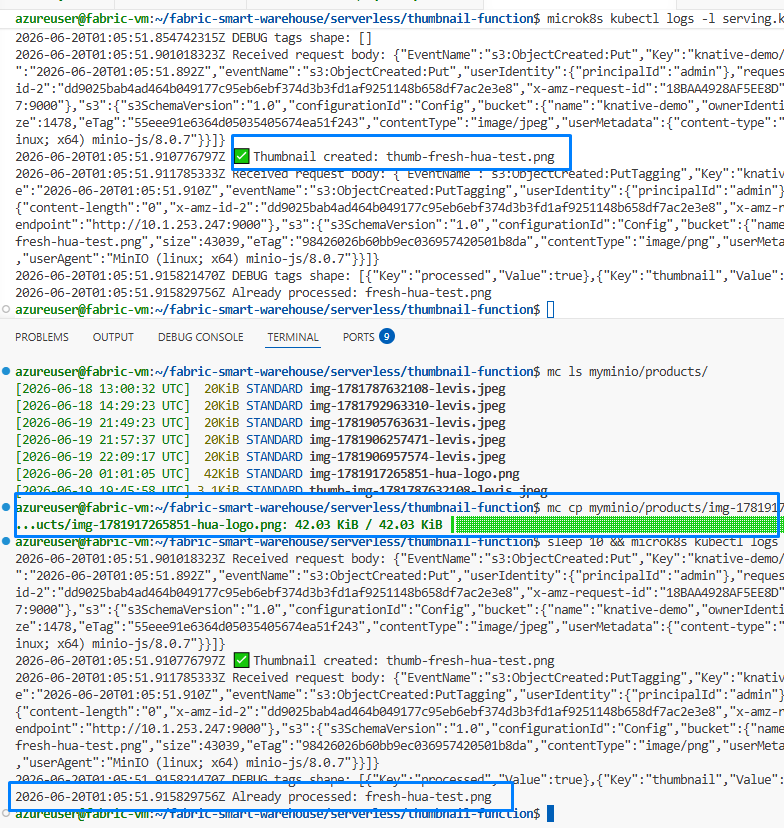
\includegraphics[width=\textwidth]{project/report/figures/knative-results.png}
  \caption{Αρχεία καταγραφής (\textit{logs}) της συνάρτησης \textit{Knative} μετά τη διόρθωση: το αρχείο επεξεργάζεται μία φορά (\textit{«Thumbnail created»}), και το επόμενο γεγονός \texttt{PutTagging} αναγνωρίζεται σωστά ως ήδη επεξεργασμένο (\textit{«Already processed»}), χωρίς νέο κύκλο εκτέλεσης}
  \label{fig:knative-fix-logs}
\end{figure}

\newpage

Το περιστατικό αυτό αναδεικνύει μια σημαντική ιδιαιτερότητα των \textit{event-driven} αρχιτεκτονικών: μια ενέργεια \textit{γραφής} --- όπως η επισήμανση ενός αρχείου --- μπορεί η ίδια να παράγει νέο γεγονός, και σφάλματα σύγκρισης τύπων σε συνθήκες προστασίας (\textit{guard conditions}) δεν εκδηλώνονται ως κατάρρευση, αλλά ως αθόρυβη, ατέρμονη επανάληψη. Ακριβώς επειδή η αποτυχία ήταν σιωπηλή, η ανίχνευσή της δεν θα ήταν δυνατή μέσα από στατική ανάλυση κώδικα --- μόνο η συστηματική παρακολούθηση της πραγματικής συμπεριφοράς, σε πραγματικό χρόνο εκτέλεσης, αποκάλυψε το πρόβλημα. Το επόμενο κεφάλαιο επεκτείνει αυτή την ανάγκη παρακολούθησης σε επίπεδο ολόκληρου του συστήματος, παρουσιάζοντας τα εργαλεία παρατηρητικότητας (\textit{observability}), τον μηχανισμό αυτόματης κλιμάκωσης, και τις πειραματικές μετρήσεις που οδήγησαν στον καθορισμό επιπέδων ποιότητας υπηρεσίας.